\scanpage{55}
\mspage{54}

bounded above by $F$ are called the \uline{strata} of $\deleted{E}F$. (Thus, \deleted{some} stratum of $F$ is a multistratum)

The set of strata of $F$ \deleted{is called} will be denoted $\overline F$ : \[ \begin{aligned} \deleted{\overline F\subset M} &\qquad  M\subset\mathcal F\\ F\longrightarrow\overline F &\qquad \mathcal F\longrightarrow\mathcal P( M). \end{aligned} \]

\uline{$\mathcal C$ 2} Every figure is the supremum of its strata : \[ F=\underset{\deleted{A}X\in\overline F}{\mathrm{Sup}}\ X \]
\figure{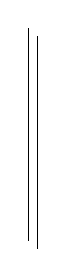
\begin{tikzpicture}\draw (0,0)--(0,2.7);\draw (.12,-.1)--(.12,2.6);\end{tikzpicture}}
\uline{Corollary} 1 The map $\deleted{X}F\longrightarrow\overline{\deleted{C}F}$ \[ \mathcal F\longrightarrow\mathcal P( M) \] is an injection, and induces an isomorphism of ordered sets of $\mathcal F$ with the set $\Phi\subset\mathcal P( M)$ formed by the $\overline F$.

This isomorphism transforms $\underset{i}{\mathrm{Sup}}$ into $\bigcup_i$
\figure{\begin{tikzpicture}\draw (0,1.5)--(0,2.8);\draw (.1,-2)--(.1,.5);\end{tikzpicture}}
\uline{Corollary 2} The set $\Phi$ of subsets of $ M$ satisfy the two conditions,

\deleted{a) $\Phi\ne\varnothing$}

% slanted
\margin{\deleted{This}} \deleted{b)}a) If $A\in\Phi$, and $(A_i)_{i\in\unsure{I|\Phi}}$ is a family of elements of $\Phi$, with $A_i\subset A$, then $\bigcup_iA_i\in\Phi$.

b) $\forall X\in M$, there exists a least $A=A_X$ such that $X\in\unsure{A|A_x|A_X}$ (a fortiori, $\Phi$ covers $ M$).
